%%% The main file. It contains definitions of basic parameters and includes all other parts.

%% Settings for single-side (simplex) printing
% Margins: left 40mm, right 25mm, top and bottom 25mm
% (but beware, LaTeX adds 1in implicitly)
\documentclass[12pt,a4paper,dvipsnames]{report}
\setlength\textwidth{145mm}
\setlength\textheight{247mm}
\setlength\oddsidemargin{15mm}
\setlength\evensidemargin{15mm}
\setlength\topmargin{0mm}
\setlength\headsep{0mm}
\setlength\headheight{0mm}
% \openright makes the following text appear on a right-hand page
\let\openright=\clearpage

% Settings for two-sided (duplex) printing
%\documentclass[12pt,a4paper,twoside,openright,dvipsnames]{report}
%\setlength\textwidth{145mm}
%\setlength\textheight{247mm}
%\setlength\oddsidemargin{14.2mm}
%\setlength\evensidemargin{0mm}
%\setlength\topmargin{0mm}
%\setlength\headsep{0mm}
%\setlength\headheight{0mm}
%\let\openright=\cleardoublepage

%% Generate PDF/A-2u
\usepackage[a-2u]{pdfx}

%% Character encoding: usually latin2, cp1250 or utf8:
\usepackage[utf8]{inputenc}

%% Prefer Latin Modern fonts
\usepackage{lmodern}

%% CUSTOMIZATION: Support diacritics
\usepackage[T1]{fontenc}
\usepackage{textcomp}

%% Further useful packages (included in most LaTeX distributions)
\usepackage{amsmath}        % extensions for typesetting of math
\usepackage{amsfonts}       % math fonts
\usepackage{amsthm}         % theorems, definitions, etc.
\usepackage{bbding}         % various symbols (squares, asterisks, scissors, ...)
\usepackage{bm}             % boldface symbols (\bm)
\usepackage{graphicx}       % embedding of pictures
\usepackage{fancyvrb}       % improved verbatim environment
\usepackage[sort&compress]{natbib}         % citation style AUTHOR (YEAR), or AUTHOR [NUMBER]
\usepackage[nottoc]{tocbibind} % makes sure that bibliography and the lists
			    % of figures/tables are included in the table
			    % of contents
\usepackage{dcolumn}        % improved alignment of table columns
\usepackage{booktabs}       % improved horizontal lines in tables
\usepackage{paralist}       % improved enumerate and itemize
\usepackage{xcolor}         % typesetting in color

\ifdefined\version\ifx\version\empty\else
	\usepackage{background}
	\SetBgContents{\version}
	\SetBgScale{1}
	\SetBgAngle{0}
	\SetBgOpacity{1}
	\SetBgColor{gray}
	\SetBgPosition{current page.south west}
	\SetBgAnchor{right}
	\SetBgHshift{.5cm}
	\SetBgVshift{.5cm}
\fi\fi

\usepackage{bold-extra}
\usepackage{wrapfig}
\usepackage{qrcode}
\usepackage{xurl}
\usepackage{float}
\usepackage{import}
\usepackage{listings}
\lstset{
  basicstyle=\ttfamily,
  columns=fixed,
  fontadjust=true,
  basewidth=0.5em,
  showstringspaces=false,
}
\definecolor{gray}{rgb}{0.4,0.4,0.4}
\definecolor{darkblue}{rgb}{0.0,0.0,0.6}
\definecolor{cyan}{rgb}{0.0,0.6,0.6}
\lstdefinelanguage{XML}
{
  morestring=[b]",
  morestring=[s]{>}{<},
  morecomment=[s]{<?}{?>},
  stringstyle=\color{black},
  identifierstyle=\color{darkblue},
  keywordstyle=\color{cyan},
  morekeywords={xmlns,version,type}% list your attributes here
}
\lstdefinelanguage{json}{
    literate=
     *{0}{{{\color{numb}0}}}{1}
      {1}{{{\color{numb}1}}}{1}
      {2}{{{\color{numb}2}}}{1}
      {3}{{{\color{numb}3}}}{1}
      {4}{{{\color{numb}4}}}{1}
      {5}{{{\color{numb}5}}}{1}
      {6}{{{\color{numb}6}}}{1}
      {7}{{{\color{numb}7}}}{1}
      {8}{{{\color{numb}8}}}{1}
      {9}{{{\color{numb}9}}}{1}
      {:}{{{\color{punct}{:}}}}{1}
      {,}{{{\color{punct}{,}}}}{1}
      {\{}{{{\color{delim}{\{}}}}{1}
      {\}}{{{\color{delim}{\}}}}}{1}
      {[}{{{\color{delim}{[}}}}{1}
      {]}{{{\color{delim}{]}}}}{1},
}
\usepackage{tikz}
\usepackage[multiple]{footmisc}
\usepackage{tikzpeople}
\usetikzlibrary{positioning}
\usetikzlibrary{shadows}
\usetikzlibrary{shapes.geometric,shapes.misc,decorations.pathreplacing,calligraphy}
\tikzset{%
  squarednode/.style={rectangle, draw=CadetBlue!60, fill=CadetBlue!5, very thick, minimum size=5mm,align=center},
  %
  module/.style={rectangle, draw=CadetBlue!60, fill=CadetBlue!5, very thick, minimum size=5mm,align=center},% as application
  dataSpecification/.style={rectangle, draw=Fuchsia!60, fill=Fuchsia!5, very thick, minimum size=5mm,align=center},% our new concept
  schema/.style={rectangle, draw=MidnightBlue!60, fill=MidnightBlue!5, very thick, minimum size=5mm,align=center},% artifact, but is schema
  artefact/.style={rectangle, draw=Periwinkle!60, fill=Periwinkle!5, very thick, minimum size=5mm,align=center},% general artifact
  document/.style={rectangle, draw=Periwinkle!60, fill=Periwinkle!5, very thick, minimum size=5mm,align=center},% general artifact
  mapping/.style={rectangle, draw=Black!60, fill=Black!5, very thick, minimum size=5mm,align=center},
  seda/.style={rectangle, draw=Gray!60, fill=Gray!5, very thick, minimum size=5mm,align=center},
  % ---
  % CIM
  % ---
  ontology/.style={rectangle, draw=RedViolet!60, fill=RedViolet!5, very thick, minimum size=5mm,align=center},% ontology or CIM
  %
  ontologyClass/.style={shape=rectangle, draw=violet!60, fill=violet!5, very thick, minimum size=5mm,align=center},
  % ----------------------------------
  % PIM entities used only to show PIM
  % ----------------------------------
  pimClass/.style={rectangle, draw=violet!60, fill=violet!5, very thick, minimum size=5mm,align=center},
  pimAttribute/.style={rectangle, draw=teal!60, fill=teal!5, very thick, minimum size=5mm,align=center},
  pimAssociation/.style={rectangle, draw=purple!60, fill=purple!5, very thick, minimum size=5mm,align=center},
  pimAssociationend/.style={rectangle, draw=pink!60, fill=pink!5, very thick, minimum size=5mm,align=center},
  % -----------------------------
  % PSM entities to show only PSM
  % -----------------------------
  generalSchema/.style={rectangle, draw=blue!60, fill=blue!5, very thick, minimum size=5mm,align=center},% equivalent to PSM
  %
  psmClass/.style={rectangle, draw=Orchid!60, fill=Orchid!5, very thick,align=center},
  psmAttribute/.style={rectangle, draw=OliveGreen!60, fill=OliveGreen!5, very thick,align=center},
  psmOr/.style={diamond, draw=Thistle!60, fill=Thistle!5, very thick,align=center},
  psmOrGroup/.style={circle, draw=Thistle!60, fill=Thistle!5, very thick, minimum size=5mm,align=center},
  psmIncludes/.style={chamfered rectangle, draw=Magenta!60, fill=Magenta!5, very thick,align=center},
  %
  human/.style={,minimum size=.8cm},
  database/.style={
      cylinder,
      cylinder uses custom fill,
      cylinder body fill=yellow!50,
      cylinder end fill=yellow!50,
      shape border rotate=90,
      aspect=0.25,
      draw
   },
  %
  cascaded/.style = {%
    general shadow = {%
      shadow scale = 1,
      shadow xshift = 1ex,
      shadow yshift = -1ex,
      draw,
      fill = white},
    general shadow = {%
      shadow scale = 1,
      shadow xshift = .5ex,
      shadow yshift = -.5ex,
      draw,
      fill = white}}}
\usepackage{ amssymb }
\usepackage[inline]{enumitem}

\theoremstyle{definition}
\newtheorem{requirement}{Requirement}
\newcommand{\requirementautorefname}{Requirement}
\newtheorem{definition}{Definition}
\newtheorem*{notation}{Notation}
\usepackage{tabularx}
\usepackage{makecell}

\usepackage{caption}
\usepackage{subcaption}
\usepackage{xcolor}
\newcommand{\td}[1]{\bigskip\par\noindent{\color{purple}#1}\par\bigskip}

%\usepackage[textcolor=purple,color=purple,bordercolor=white,backgroundcolor=white,size=tiny]{todonotes}\marginpar{left}
%\reversemarginpar
%\geometry{marginparwidth=75pt}
\usepackage[super]{nth}

\usepackage{afterpage}
\usepackage{pdflscape}
\usepackage{dsfont}
\usepackage{xhfill}
\usepackage[skins]{tcolorbox}
\usepackage{varwidth}
\makeatletter
\newtcolorbox{mybox}[1][]{
  enhanced,
  colframe=black, colback=white,
  sharp corners,
  boxrule=0.6pt,
  detach title,
  coltitle=black,
  colbacktitle=white,
  fonttitle=\footnotesize,
  enlarge left by=-8mm,
  enlarge right by=-2mm,
  width=\linewidth+10mm,
  left=7mm,
  right=2mm,
  before upper=\setlength{\parindent}{17.62482pt}\everypar{{\setbox0\lastbox}\@minipagefalse\everypar{}},
%  overlay={
%    \node[rotate=90,
%          fill=tcbcolbacktitle,
%          font=\kvtcb@fonttitle,
%          minimum width=1cm]
%          at (frame.west)
%      {\begin{varwidth}{\tcbtextheight}%
%         \centering\tcbtitle\par
%       \end{varwidth}};
%  },
#1}
\makeatother

% \newenvironment{showcase}
% {\bigskip\begin{mybox}[title=Example]}
% {\end{mybox}\bigskip}

\newenvironment{showcase}
{\bigskip}
{\bigskip}


%%% Basic information on the thesis

% Thesis title in English (exactly as in the formal assignment)
\def\ThesisTitle{Model-driven approach for data schema definitions modeling}

% Author of the thesis
\def\ThesisAuthor{Bc. Štěpán Stenchlák}

% Year when the thesis is submitted
\def\YearSubmitted{2022}

% Name of the department or institute, where the work was officially assigned
% (according to the Organizational Structure of MFF UK in English,
% or a full name of a department outside MFF)
\def\Department{Department of Software Engineering}

% Is it a department (katedra), or an institute (ústav)?
\def\DeptType{Department}

% Thesis supervisor: name, surname and titles
\def\Supervisor{doc. Mgr. Martin Nečaský, Ph.D.}

% Supervisor's department (again according to Organizational structure of MFF)
\def\SupervisorsDepartment{Department of Software Engineering}

% Study programme and specialization
\def\StudyProgramme{Computer Science - Software and Data Engineering (N0613A140015)}
\def\StudyBranch{Computer Science - Software and Data Engineering}

% An optional dedication: you can thank whomever you wish (your supervisor,
% consultant, a person who lent the software, etc.)
\def\Dedication{%
This thesis was made possible thanks to numerous people who helped me or motivated me during the journey.

On the one side, I would like to thank my family for the financial support and for encouraging me to continue educating myself. Thanks to my girlfriend Kateřina for all the emotional support despite the long nights spent on this project.

I want to express my gratitude to my supervisor, doc. Mgr. Martin Nečaský, Ph.D., for guiding me through this and other projects during my study and helping me find the right branch of informatics I enjoy exploring. I also value the help from my consultants Mgr. Petr Škoda, Ph.D. and RNDr. Jakub Klímek, Ph.D.

Finally, I want to thank my friend Jáchym Bártík for the encouragement and the long-lasting friendly rivalry, which will continue in our Ph.D. study.
}

% Abstract (recommended length around 80-200 words; this is not a copy of your thesis assignment!)
\def\Abstract{%
This work analyzes, formalizes, and implements a framework for multi-level conceptual modeling of various serialization formats based on Model-Driven Architecture and previously developed tools XCase and eXolutio. It enables users to model their schema from a conceptual model in one general form from which multiple schema formats can be derived alongside documentation and transformation scripts. The thesis introduces base formalisms and findings and analyzes advanced requirements for the following work in this area, such as evolution and inheritance of schemas.

The primary use case of the tool is modeling formal open standards for publishing open data for the government and public institutions of the Czech Republic. Nevertheless, the intent is to make the tool for general schema modeling.
}

% 3 to 5 keywords (recommended), each enclosed in curly braces
\def\Keywords{%
{schema definition} {data modeling} {ontologies} {Model-Driven Architecture}
}

%% The hyperref package for clickable links in PDF and also for storing
%% metadata to PDF (including the table of contents).
%% Most settings are pre-set by the pdfx package.
\hypersetup{unicode}
\hypersetup{breaklinks=true}

% Definitions of macros (see description inside)
\include{macros}

% Title page and various mandatory informational pages
\begin{document}
\include{title}

%%% A page with automatically generated table of contents of the master thesis

\tableofcontents

%%% Each chapter is kept in a separate file
\chapter*{Introduction}
\addcontentsline{toc}{chapter}{Introduction}
% Chci to mít na 4 strany

During the software development process, we may come to a point where splitting a large codebase into smaller, well-defined chunks is necessary to maintain the growth of our software. Using existing systems and connecting them is also a viable approach to building software. In both cases, we end up with many applications and services working together.

This approach reduces complexity and demands on software developers as each part can be maintained, deployed, and tested separately. Each developer team must know only the portion they maintain and the immediate surrounding. The surrounding is then defined by a protocol - the interface specifying the data which flows between the systems.

Those protocols must be created, documented, and maintained, which can be a long, error-prone task. The result of the process is usually a set of data schemas and documentation for developers. Especially the schemas need to be designed carefully to be, if possible, consistent in format and naming.

\bigskip

As an example, consider a company selling and distributing its own goods. The goods are stored in warehouses and then shipped to customers. For the shipping process, the warehouse workers need to know the properties of items they need to send. Similarly, customers need to know the properties of items they are buying. This scenario is denoted in the following image. The nodes are individual systems in the company that communite with each other.

\begin{figure}[h]\centering
\begin{tikzpicture}[
    squarednode/.style={rectangle, draw=purple!60, fill=purple!5, very thick, minimum size=5mm},
]
    %Nodes
    \node[squarednode] (db) {Company's goods database};
    \node[squarednode] (warehouse) [below=2cm of db, xshift=.5cm,anchor=north west] {Warehouse application};
    \node[squarednode] (shop) [below=2cm of db, xshift=-.5cm,anchor=north east] {Online shop};

    %Lines
    \draw[-latex] (db) -- node[text width=3cm,align=center,auto,anchor=west,midway]{order info with items to send} (warehouse);
    \draw[-latex] (db) -- node[text width=3.5cm,align=center,auto,anchor=east,midway]{list of available items} (shop);
\end{tikzpicture}
\end{figure}

Our goal is to describe the protocols formally. Which data are sent and where. By doing this without any tool, we may find several obstacles during the process:

\begin{enumerate}
    \item We may need to describe an entity for every schema that uses it. Hence doing the \textbf{same work multiple times}.
    \item There is a high chance of \textbf{incostinency}. We may name the semantically same attribues differently which may cause confusion among software enginners who came in touch with multiple parts of the system.
    \item We \textbf{lack of context} in the whole system where the entities are used.
\end{enumerate}

In addition to these obstacles, it is hard to provide supporting documentation, diagrams and examples. Future modifications to the system may require changing the schemas, which again may require changing same thing multiple times and may cause inconsistency. Formally, we will denote changing of schemas as an \textbf{evolution}.

\section*{Ontology}
\addcontentsline{toc}{section}{Ontology}

The example above tends us to create a formal description and naming of all entities, their properties and relations in the given domain. Entities represents objects from a real world, such as \textit{order}, \textit{customer} or \textit{goods}. Relations then specify for example that \textit{order belongs to a customer} and \textit{consists of goods}. Formally, such description is called an \textbf{ontology}.

With the data on the web \cite{data-on-the-web} trend in the last few years, even ontologies are becoming accessible publicly. Popular formats include RDFS (or RDF Schema), OWL, UFO, or schema.org and Wikidata. For example, schema.org is a proprietary format describing usefull data for search engines, such as events, organizations or places.

Using pre-defined ontologies in semi-automatic way of defining schemas is beneficiary, because a schema designer may focus fully on the schema structure and not on the domain semantics.

\section*{OFNs and open data}
\addcontentsline{toc}{section}{OFNs and open data}

\textbf{Open data} is defined as data published on the web without any restrictions on use. This means, than anyone can use, modify and distrubute the data under any reason, including commercial use.

Definition of open data is very loose, but can be further specified by a 5-star scheme designed by Sir Tim Berners-Lee. Each star adds a restriction up until the fifth star describing the Linked Open Data.
\begin{itemize}[noitemsep,leftmargin=2cm]
    \item [1 $\bigstar$] Data are published on the web and can be used freely.
    \item [2 $\bigstar$] Data are structured and in machine-readable format.
    \item [3 $\bigstar$] The format is not proprietary, hence anyone can open them.
    \item [4 $\bigstar$] Data uses RDF and SPARQL standards from W3C.
    \item [5 $\bigstar$] Data are linked to other data creating a network of data.
\end{itemize}

\smallskip

According to Act 106/1999 Coll. of the Czech Republic, data of public institutions shall be published as open data on the Internet in all formats it was created, and if possible, in a machine-readable format. This description corresponds to two stars in the schema above.

The act then specifies \textbf{OFNs}\footnote{\url{https://data.gov.cz/ofn/}} \textit{(open formal norms)} as recommendations for publishing selected types of data, such as information about \textit{Tourist destinations} and \textit{Sports centers}. The purpose of these documents is to standardize how these data are published, usually by defining JSON and XML schemas along with textual documentation.

Until recently, all those recommendations (OFNs) were created by hand without any tool.

\smallskip

The process of designing those recommendations is comparable to designing schemas for a software system mentioned above - the designer needs to create schemas and documentation for them with examples and images.

\newpage
\section*{Focus of the work}
\addcontentsline{toc}{section}{Focus of the work}

This thesis will analyze and extend\footnote{The author implemented the basis of the tool as his research project. This thesis, therefore, introduces advanced constructs and only formalizes those already implemented.} a newly created tool, Dataspecer \cite{dataspecer}, and formally define and analyze its internal model, which follows previous research in the XML data modeling area and extends it to support new requirements.

Dataspecer is a web tool for effortless creation and management of data specifications, such as XSD, JSON Schema, and CSV Schema, and the creation of supplementary documents. The tool helps the user model schemas by providing relations from the chosen ontology. Schemas are modeled in a graphical interface in the form of the tree, which is then converted to various schemas.

Supplementary documents are automatically generated files from the modelled schemas, such as:

\begin{itemize}
    \item \textbf{documentation} - Human-readable description of entities from the ontology, that are used in the schema as well as description of the schema.
    \item \textbf{data transformations} - Scripts that can convert data from one schema to another, even between different technologies, such as JSON and XML.
    \item \textbf{examples} - Small datasets that can be used instead of the documentation to understand the schema.
    \item \textbf{example application} - Depending of context of modelled schema, if the schema describes a web accessible data, it is possible to generate a web application that uses those data as an proof that the workflow works.
\end{itemize}

The tool is already in use for creating new schemas for the public sector of the Czech Republic including the OFNs.

\bigskip

\noindent The rest of the thesis is organized as follows.

\begin{itemize}
    \item The following chapter \ref{chapters:related-work} analyzes related work and introduces the previous works as the common ground this work will follow - specifically the model-driven approach for data modeling and evolution of XML documents.
    \item Chapter \ref{chapters:analysis} briefly analyzes new requirements for the software as many requirements were already studied in the related work. The chapter focuses on support for schemas other than XML and the data on the web \cite{data-on-the-web} approach to ontology and the modeled schemas.
    \item Formal background (chapter \ref{chapters:formal-background}) then defines the internal model to represent schemas and its changes from the related work where it was first introduced. Changes are also analyzed with respect to the new requirements.
    \item The next chapter \ref{chapters:implementation} then briefly describes how this model is integrated into the Dataspecer tool.
    \item The last chapter \ref{chapters:future-work} introduces and briefly analyzes topics for future work, such as the change propagation (evolution) in schemas.
\end{itemize}


\chapter{Previous research}
\label{chapters:previous-research}

This short chapter introduces the core concepts of the previous research that was carried out by the \textit{XML and Web Engineering Research Group} (XRG) at the Faculty of Mathematics and Physics of the Charles University in the years 2012 to 2015. Those concepts will be used for further analysis in the following chapters.

\bigskip

In 2012 XRG formalized a novel approach\footnote{The work builds on previous work of the same authors where they introduced the XSEM model \cite{necasky2007xsem}, which has later been a subject of their study.} to modeling XML schemas \cite{necasky2012conceptual} for a particular domain ontology by integrating Model Driven Development \cite{kent2002model} (specifically Model Driven Architecture) techniques to separate a conceptual mo\-del describing the domain ontology and a structural model which described the concrete XML schema.

\paragraph{Model-Driven Architecture} MDD is a software engineering technique that abstracts software development into several levels (models) to allow flexibility by separating business domain from platform decisions. MDA \cite{mda,mda_developing_in} introduced by Object Management Group (OMG) is a specialization of MDD focusing on the automation of the development of software systems.

MDA introduces four models. The topmost level CIM (Computation Independent Model) expresses the business logic and has no formal representation, as it is only a concept, hence the name computation independent. PIM (Platform Independent Model) as a second level models the business logic in UML. It does not specify a concrete platform or technology, but only the concepts in a formalized way. PSM (Platform Specific Model) reflects the formalized concepts from PIM in a platform-specific environment, such as in XML Schema, C\# or Java code, or a database schema.

The key concept is a transformation as the process of mapping the upper layer to the lower one. The transformation from CIM to PIM must be done by hand as CIM does not formally exist. More interesting is PIM to PSM transformation, as it can be automated. The transformation keeps the mapping to preserve the semantics between the models. The last level is Implementation Specific and only represents different implementations of PSM.

\bigskip

XRG used PIM and PSM in their architecture. PIM represented the domain ontology in UML-like notation\footnote{Formal definition of PIM and PSM levels is in chapter \ref{chapters:formal-background}.}, as it is independent of the platform as XML. PSM\footnote{Compared to the definition above, XRG's PSM is more like the mapping between the PIM and PSM from the MDA. Final XML Schema would then corresponds to PSM.} then represented the given schema in their own designed grammar, which was translated into a final schema, such as XSD.

\begin{figure}[h]\centering
    \begin{tikzpicture}
        %Nodes
        \node[ontology] (pim) at (0,0) {PIM schema};
        \node[generalSchema] (psm1) at (-2.5,-1.5) {PSM schema 1};
        \node (psmDot) at (0,-1.5) {...};
        \node[generalSchema] (psmN) at (2.5,-1.5) {PSM schema N};

        \node[schema] (schema1) at (-2.5,-3) {XML schema 1};
        \node (psmDot) at (0,-3) {...};
        \node[schema] (schemaN) at (2.5,-3) {XML schema N};

        \node[document,cascaded] (q1) at (-1.5,-4.5) {XML queries};
        \node (psmDot) at (1,-4.5) {...};
        \node[document,cascaded] (qN) at (3.5,-4.5) {XML queries};

        \node[document,cascaded] (document1) at (-2.5,-6) {XML documents};
        \node (psmDot) at (0,-6) {...};
        \node[document,cascaded] (documentN) at (2.5,-6) {XML documents};

        \node (psm_t)[text width=4cm,align=right] at (-7,0) {{Platform-specific level:}};
        \node (pim_t)[text width=4cm,align=right] at (-7,-1.5) {{Platform-independent level:}};
        \node (schema_t)[text width=4cm,align=right] at (-7,-3) {{Schema/Logical level:}};
        \node (ext_t)[text width=4cm,align=right] at (-7,-4.5) {{Operational level:}};
        \node (ext_t)[text width=4cm,align=right] at (-7,-6) {{Extensional level:}};

        %Lines
        \draw[-latex] (psm1) -- (pim);
        \draw[-latex] (psmN) -- (pim);
        \begin{scope}[transform canvas={xshift=-2em}]
            \draw[-latex] (document1) -- (schema1); % node[fill=white]{conforms}
            \draw[-latex] (documentN) -- (schemaN); % node[fill=white]{conforms}
        \end{scope}
        \draw[-latex] (schema1) -- (psm1);
        \draw[-latex] (schemaN) -- (psmN);
        \draw[-latex] (q1) -- (schema1);
        \draw[-latex] (qN) -- (schemaN);

        % separators
        \foreach \x in {0,...,3}{
            \draw [dotted] (-9,-0.75-1.5*\x) -- (5,-0.75-1.5*\x);
        }
    \end{tikzpicture}
    \caption{The five-level framework proposed by XRG in \cite{necasky2012conceptual}. A shared PIM layer with a conceptual model is used by multiple PSMs, where schemas are defined in their own grammar. The grammar is then translated into schemas that conform to XML documents in the last level.}
\end{figure}

The major benefit of the strategy presented is a shared conceptual model between various XML schemas, as other works at that time had a conceptual model for every schema. This was not practical as usually multiple schemas are applied in a single software. Authors have also formalized the model and have proven that their approach is correct. That means that (i) every conceptual schema models XML schema, (ii) their translation algorithm from the internal model to schema respects introduced rules and is reversible, and (iii) their normalization and optimization algorithms produce semantically same schema.

\begin{figure}[h!]
    \centering
    \includegraphics[width=\textwidth]{img/exolutio.png}
    \caption{Preview of the eXolutio tool. The left panel shows the PIM model as a UML class diagram, while the right panel represents a PSM schema in a tree-like structure that can be converted to an XML schema.}
    \label{fig:exolutio}
\end{figure}

Their primary use case was to create schemas for the government, such as the information system for National Register for Public Procurement (NRPP) for publishing public contracts.

\paragraph{Modeling} To create a schema, a user has to first create an ontology of desired entities as PIM. Then, multiple schemas can be created as PSM trees by first selecting a schema root and then adding entities to it. The resulting XML schemas then can be exported from the application.

\paragraph{Evolution of schemas} The focus of XRG was also directed to the evolution \cite{nevcasky2012evolution} of their proposed model to minimize the work of the data designer. As already stated in the introduction of the thesis, changes may be inevitable (either from the user requirements or from the surrounding environment) in large and complex systems, and propagating even a tiny change from the domain ontology to all affected schemas is time-consuming and error-prone.

They proposed, formalized, and later implemented a solution in restricting the changes in PIM and PSM models to only atomic operations - simple changes in the model, such as \textit{creating a new class}, \textit{updating a name of association} or \textit{removing an attribute}. Those operations are not intended to be used by the user directly but are simple enough to be formally defined and mapped to the corresponding operations in the level below. The proposed mapping is then used to propagate changes in the model to the schema level, more precisely from PSM to PIM, which is then translated to the schema level. They implemented only top-down propagation of changes as the propagation from XML documents is usually not meaningful (but theoretically possible).

\paragraph{Implementation} Their result were implemented in two tools \textit{XCase} \cite{xcase} and \textit{eXolutio} \cite{exolutio}. The former one was simpler, focused only on modeling. The latter then supported schema evolution as described in the previous section. Tools let users define the ontology from which the schemas and operations were derived for XML documents.

\paragraph{Analysis} The tool was designed only for XML, hence is not usable for other languages, such as JSON, which is very popular at the time of writing this thesis as being used by many server-centered applications to communicate with the server through the REST API \cite{fielding2000architectural}, for no-SQL databases\footnote{\url{https://www.mongodb.com/}}\footnote{\url{https://rethinkdb.com/}} and more. Nevertheless, we can use their findings and generalize the model for other formats.

They focused on the correctness and completeness of the model, which in some cases may be a limitation, such as more complex implementation and processing of the model to not allow a user to create a schema that is not valid.

Lastly, the tools didn't support sharing and collaboration, as at that time this was not considered standard practice in the industry.
\chapter{Analysis and formal description of CIM and PIM layers}
\label{chapters:analysis}

\begin{requirement}
    \label{requirement:ontologies-on-the-web}
    As many ontologies are located on the web in formats like OWL, RDFs, UFO and etc.,
    \begin{enumerate*}[label=\textit{(\alph*)}]
        \item the application must support reading them.
        \item The previous approach of creating the ontology directly in the application is not required, but there should be a support for \textit{some} modifications.
      \end{enumerate*}
\end{requirement}

In contrast with the approach introduced in \textit{XCase} and \textit{eXolutio} tools, the process of creating the domain ontology is moved from the application to the extednal tools. The application then only uses those existing ontologies in standart situations.

Before we proceed to formal description, lets focus on impacts of first part of the requirement.

\begin{enumerate}
    \item The ontology may \textbf{not be always avaiable}. This should not forbid us to generate the schemas and make small changes in the schemas if those changes are not directly related to reading the ontology.
    \item The ontology may \textbf{change unexpectedly}. As there are no strict requirements, we must not expect to get the history of changes, yet still be able to perform schema evolution in some semi-automatic way.
    \item The entities in the ontology may \textbf{point to another ontology} according to Linked Open Data principles.
\end{enumerate}

To support \nth{1} and \nth{2} point, the previously introduced five-level framework was modified. We have added new top-most level called CIM (from \textit{Computational Independent Model}). CIM represents the domain ontology. Although there can be more ontologies, with LOD approach we can see them as one. PIM is then used as a copy of CIM and only the necessary entities are copied to PIM. This modification is in accordance with point 1 and gives us base ground for implementing point 2, as we can compare CIM and PIM and try to create a sequence of operations that modifies PIM to be consistent with CIM.

\begin{requirement}
    \label{requirement:multiple-technologies}
    The application shall support multiple serialization technologies (such as JSON Schema, XSD and CSV schema) and it shall be possible to easily add support fot other.
\end{requirement}

Although the requirement \ref{requirement:multiple-technologies} mainly affects the PSM level, it has also impact to the definition of ontology. As we shall support all kinds of serialization technologies, some of them may not use all the information, which forces us to define the ontology and PIM layer in simpliest, most elementary way.

\begin{definition}[PIM] PIM is a triple $S=(S_c, S_a, S_r)$ of sets of classes, attributes and associations, respectively such that:
\begin{itemize}
    \item Attribute $A \in S_a$ belongs to class $C \in S_c$, which is denoted by function $\textrm{class}: S_a \rightarrow S_c$ as $\textrm{class}(A)=S$.
    \item Association $R \in S_r$ is a set of exactly two association ends ${E_1, E_2}$ that are associated with classes similarly as with attributes by $\textrm{class}: E \rightarrow S_c$.
\end{itemize}
\end{definition}

PIM then can be decorated by various semantic and syntactic anotations:

\begin{itemize}
    \item Classes, attributes, associations and association ends may have title and description, or potentially other describing properties that are not directly used in schema generation. However, the title may be used to propose naming of entities' labels in the PSM level.
    \item Attributes and association ends have cardinalities.
    \item Attributes have data types.
\end{itemize}

\begin{definition}[CIM]
CIM $O$ is an ontology database for which function \textit{CIM adapter} $A$ exists, such that $A(O) = S$ is a valid PIM, where every entity $I$ has unique interpretation $interpretation(I)$. Interpretations must be stable and consistent.
\end{definition}

The definition tells us, that CIM is everything that can be translated to PIM and that process is stable over time. If CIM is slightly changed, also the resulting PIM will be changed only slightly. If CIM is stored in LOD format, than the $interpretation$ function returns the URI of the CIM entity, that corresponds to the given PIM entity.

For simplification, in the rest of the thesis we may ommit that CIM "needs to be translated" to PIM and suppose that is already in PIM-like format.

\begin{definition}[consistency]
    We say that \textbf{PIM is consistent with CIM}, if PIM is a subset of CIM.
\end{definition}

From the descriptions above, the inconsistency may happen only if the CIM changes. It is easy to detect it as we can compare entities in PIM with those in CIM. To support the \nth{2} point from requirement \ref{requirement:ontologies-on-the-web}, we would need to create a set of atomic operations on the PIM level that make the PIM consistent again. These operations can be propagated up to schemas to apply the change from the ontology.

\section{User modifications on the PIM level}

As stated in the requirement \ref{requirement:ontologies-on-the-web}, the usual scenario for data modelling consists of reading an ontology from the web as a CIM. This section analyzes the second part of the requirement, whether there exists scenarios, where modifying the ontology in the tool may be beneficial than modification of the ontology itself.


We can classify the reasons for modifying the ontology as follows:

\begin{enumerate}
    \item The ontology is wrong and does not describe the domain correctly. - \textit{Then the most correct way would be to fix the ontology.}
    \item The ontology describes only a subset of the domain. Either only the core of the domain, or the ontology is complete, but only for one domain, whether in another, something may missing. - \textit{If the desired ontology is strictly a superset of the domain, we can exploit the features of linked data to add missing anotations in our own structured data. Then, we would use the new ontology.}
    \item The ontology is not granular enough. Some entities can be represented in more details than currently are. - \textit{We would need to create a copy of affected classes or use advanced tool, if exists.}
\end{enumerate}

Suppose the example with goods in the delivery company. Although the goods may be identified by EAN (barcode on items), the software team may prefer the other, iternal identifiers. There can be reasons for not including the identifier into the ontology, as it is too internal or specific for only a software team. That would correspond to the second category. The third category may represents the case, when we need to replace an address with a set of more specific attributes such as \textit{street}, \textit{number}, \textit{city}, \textit{country}, etc.

Although in all the scenarios, the preffered way would be to create a new ontology, it can be too cumbersome and time consuming. Therefore, it should be possible to somehow allow modifying the PIM. PIM, that has been modified will be denoted as "user PIM" or \textbf{UPIM}.

\bigskip

In context of other requirements and the framework used, this would also mean that:
\begin{itemize}
    \item PIM that is not consistent with CIM and we do not intent to make it consistent can be "marked" as UPIM. This would stop proposing the user to evolute the schemas according to the newest CIM.
    \item If CIM changes, the semi-automatic update can respect UPIM and ask the user for changes, that can not be performed automatically.
\end{itemize}

We propose to add UPIM to the framework as a new level between PIM and PSM. The purpose of UPIM will be modyfying the ontology stored in PIM by adding, or overwriting the entities.

Construct used in UPIM must be chosen wisely as we do not wont to create too complex ontologies that will be hard to maintain both by user and the evolution mechanism. Yet, it is prefered to give user more freedom than restricted, but more formal and stable model.

We allow all constructs from PIM as it shoud be definitelly possible to move everything from PIM to UPIM.
\chapter{Formal background} - formalni popis vrstev
\label{chapters:formal-background}

\section{CIM layer}

\begin{itemize}
    \item Definition by PIM (must be stable, function from CIM to PIM)
    \item Antidefinitions, how we use interpret it (changes, not available)
\end{itemize}

\section{PIM layer}

\begin{itemize}
    \item Why this PIM - maybe link to UFO?
\end{itemize}

\subsection{user PIM}

\begin{itemize}
    \item definition, analysis, implementation
\end{itemize}

\section{PSM layer}

\begin{itemize}
    \item General definition - most unique
    \item analysis of basic constructs that may be used, OR and INCLUDE analysis
    \item News compared to old version - reuse
\end{itemize}
\chapter{Implementation}\label{chapters:implementation}

This chapter aims to provide implementation details of the fundamental concepts introduced during the analysis in \autoref{chapters:analysis} and formalized in \autoref{chapters:formal-background}, hence closing the reasoning process. Its purpose is not to replace complete technical documentation or provide a basic architectural structure.

\bigskip

The intent of the work is to build a solid foundation for an ecosystem of tools with the core framework for schema modeling. The key elements that shall be followed to achieve this goal are:
\begin{enumerate}
    \item All model data and configuration shall be stored in RDF - \textit{There is already an ecosystem of tools that can work with RDF. It is easily shareable and linkable.}
    \item The core framework shall work on its own - \textit{It shall be possible to integrate into other applications. The tool is only a user-friendly interface to execute the framework.}
    \item Generators shall work as plugins for the core framework - \textit{The idea is that anyone can design generators for their specific purpose.}
    \item The model shall be robust and extensible
\end{enumerate}

Due to the current use case and state of development, our primary focus is to create a tool where is easy to design schemas and generate the required artifacts. Hence the goals above are not met yet, but some design decisions were made to fulfill them later easily.

\section{Model representation}

\subsection{Store}

As model data are represented by entities that shall be serialized in RDF, we introduce a \textbf{schema store} as an abstraction layer. The schema store can read and write \textbf{resources}, where the resource is a document/object that contains arbitrary data. In the context of PIM and PSM, the entity is a resource. Resources are identified by their IRI, which is an IRI of the corresponding RDF resource.

Entities can be read from the schema store, but writing is limited to \textbf{operations}. Operations that were executed are saved in the schema store to provide a history of the model at any given point in time. Schema store must contain exactly one \textbf{schema resource}. A schema resource is a resource that identifies all other entities in the schema store, formally creating a set of resources.

Schema stores are managed in \textbf{stores}. The store is an interface for reading resources by their IRI and executing operations on a given schema resource. The store is asynchronous and represents a database of resources. For example, a store may be an interface on the SPARQL endpoint, a file system, a read-only dump on the internet, or just data in local memory.

The current implementation of the tool uses stores that are synchronized with the server through a simple GET-POST API.\footnote{This de facto implicitly supports Solid Pods as a type of store.} Stores on the server are saved into individual files in the filesystem. Each store contains only one schema store for better granularity, as the file must be read and written atomically.

\medskip

The store also shall generate new IRIs that can be later assigned to entities. IRIs needs to be generated in advance to be part of the operation, so we can later identify which entities were created. Depending on the store, the IRIs may have different structures.

The current implementation only supports a simple reading by IRI. This will be changed in the future for more advanced query operations, such as reverse lookup for the entity.

\medskip

Stores' interface allows creating of \textbf{federated stores}, hence allowing to have only a single interface for reading and writing any entity. This simplifies the application's design, as we may have a complex system of shared and reused data specifications from different sources.

\medskip

In previous chapters, we have considered PIM as both the layer in general (PIM layer) and the set of PIM entities we have formally defined (PIM schema). The latter one, the PIM schema, is represented by one specific schema store. Similarly, the PSM schema (possibly having multiple roots) is also represented by one schema store. To simplify the design, the schema resource that is necessary for every schema store will also represent the PIM or PSM schema. To make the previous sentence clear, suppose PSM schema $S$. The schema contains entities such as classes, ORs, etc. Those entities are represented by resources. But the schema itself, which contains, for example, a set of roots, also needs to be represented by a resource. And the resource will be the schema resource.

This means that if a user creates a data specification with two schemas, three schema stores are created: one for the PIM schema and two for the PSM schemas. Hence three stores represented by three files are created as well.

\subsection{Data specification}

The resource that represents data specification contains, namely, (i) a set of reused data specifications' IRIs, (ii) a set of PIM schemas' IRIs, (iii) a list of PSM schemas' IRIs, (iv) a set of stores' IRIs where the appropriate schemas can be found and (v) an artifact configuration.

\section{Layers for simplifying the model}

Reading the model may be too complex, as the entities may not exist, reading them requires asynchronous access, and to obtain the value of all annotations, we usually need to go to the PIM layer. Letting individual generators access the model is, of course, necessary, but for most generators, this would mean implementing many helper functions for easier access. To reduce the burden on generators, we introduce conceptual and structural models whose purpose is to provide a more user-friendly interface for reading the model.

\paragraph{Conceptual model} Conceptual model is fairly simple as it only simplifies access to PIM, which is simple by itself. Its structure is similar to PIM, but attributes and associations are referenced directly from the class as properties. The whole model is constructed in advance, hence we can check whether is correct, but mainly we can access everything synchronously.

\paragraph{Structural model} Structural model employs a different approach to schema structure than PSM. As PSM is highly inspired by schemas, it also has a more schema-like structure. For example, include is valid class property, but from an object-oriented view, it has more semantic meaning. The structural model we use tends to be more object-oriented.

Classes have properties as well, but the properties represent only attributes and associations. Include is translated to class inheritance, as it works almost precisely the same as inheriting properties from a parent class. The only difference is that the position of the include can not be preserved. This, however, for most generators, is not an issue.

To simplify the work with disjunction, we exploit the fact that OR on one element is the same as the element without OR. Hence, all associations have an array of referred classes. This won't introduce new objects that need to be specially handled and allows domain-specific generators to ignore the concept at all if it is not required.

\paragraph{Transformations} Both conceptual and structural models provide various transformations (do not confuse with data transformations from \autoref{req:transformations}) that simplify the model or obtain additional data.

\begin{itemize}
    \item It is possible to flatten the structural model by copying properties from parent to child classes. This transformation may simplify the work for developers of generators as they do not need to handle inheritance anymore. Of course, this would cause the artifact to grow as the entities are not reused but may be useful for an early stage of development as simplification.
    \item As some information lies in PIM, such as naming, description, default cardinality, or datatype, there is a transformation that fetches this information to the structural model.
    \item Associations marked as dematerialized may be "unpacked" to the parent class instead of the association itself.
\end{itemize}

\paragraph{Format-aware structural models} As there is usually a whole ecosystem of generators that work with a given technology, such as XML, it is important to let the designers extend or even transform the model on their own, making it format-aware. We already use this technique for XML to add namespace information to the entities. In general, the transformation may change the interface of the structural model to suit the needs of the generator better.

\chapter{Related work}
\label{chapters:related-work}

\section{OSLO}

OSLO\footnote{\url{https://joinup.ec.europa.eu/collection/oslo-open-standards-linked-organisations-0/about}} - Open Standards for Linked Organisations is an initiative that originated in Flanders, Dutch-speaking northern portion of Belgium, to promote the use of technical standards for the data exchange between various organizations, government, and a local government. The goal of OSLO is to maintain and create the standards through the open process (hence everyone can intervene), keep the rules respected, provide a publication platform and support the adoption of the standards. So far, OSLO contains over 18 different domains consisting of definitions from 107 organizations.

The initiative developed a toolchain to ease the process of publication of the standards. The standards are modeled in \textit{Enterprise Architect UML} software and then converted into an RDF representation with their tool\footnote{\url{https://github.com/Informatievlaanderen/OSLO-EA-to-RDF}}. The next tool then generates artifacts (resulting files) that are automatically published on one centralized server \url{https://data.vlaanderen.be/ns}. The artifacts contain HTML documentation, RDF vocabulary, SHACL\footnote{\url{https://www.w3.org/TR/shacl/}} templates for validation of RDF, and a JSON-LD\footnote{\url{https://json-ld.org/}} context for developers that prefer JSON formats. Their toolchain uses the GitHub platform for storing their standards and triggering the rest of the toolchain. They also provide tools for organizations to validate their data against the standards to check that data are machine-readable without errors.

OSLO also focuses on the interoperability of services that provide those data so that every service has a generic hyper-media-driven API.

\medskip

Compared to our approach, OSLO's primary focus is on the interoperability of public services and their data in LOD format. Their goal is to provide a set of tools to create and later validate public services effectively. Our approach is to design a general tool (hence it can be used for any related purpose, such as software development process) for services that use non-RDF formats, such as CSV or XML files, and provide tools to convert them to linked data format.

As noted in the introduction chapter, we also focus on the public sector, but only as one of many use-cases. Hence, in general, their approach is better suited for the public sector as their tool may be better suited to the problem.

\section{LinkML}

LinkML is a general-purpose language and a tool using YAML for modeling schemas that can be converted to various formats such as JSON, CSV, SQL and RDF schemas, or Python Dataclasses. It also generates human-readable documentation with diagrams and can validate the data in different formats. It is written in Python.

\begin{figure}[h!]\centering
    \begin{Verbatim}[commandchars=\\\{\}]
classes:
  Person:
    attributes:
      id:
        identifier: true
      full_name:
        required: true
        description: name of the person
      aliases:
        multivalued: true
        description: other names for the person
      phone:
        pattern: "^[\textbackslash{}\textbackslash{}d\textbackslash{}\textbackslash{}(\textbackslash{}\textbackslash{})\textbackslash{}\textbackslash{}-]+$"
      age:
        range: integer
        minimum_value: 0
        maximum_value: 200
    \end{Verbatim}
    \caption{Example of part of the YAML configuration file for LinkML.}
\end{figure}

The core concepts in their model are classes with properties. Classes then support inheritance and the model in general supports many options for the data types, cardinalities, regular expression patterns, and others.

Nevertheless, the main input of the framework is the YAML file where the ontology needs to be defined and then the tool generates artifacts. This is a completely different concept than we have, as the ontology already exists and we model the schemas. It seems, that the tool does not let the user choose what to include to the schema in such granularity as our tool does.

Based on how the framework is used, we suppose, that it targets the former use-case from the introduction: to create schemas for (micro)service architecture. The lack of UI makes it difficult to use outside this case.

\afterpage{\begin{landscape}\thispagestyle{empty}
  \begin{table}\centering
  \begin{tabular}{l|ccccc}\toprule
    & \textbf{OSLO} & \textbf{LinkML} & \textbf{\begin{tabular}[c]{@{}l@{}}Enterprise\\ Architect\end{tabular}} & \textbf{\begin{tabular}[c]{@{}l@{}}XCase \&\\ eXolutio\end{tabular}} & \textbf{Dataspecer} \\\midrule
  Shared ontology         & yes   & with toolchain & no                    & no                & yes               \\
  Custom schema structure & yes   & no             & no                    & yes               & yes               \\
  Schema extension        & ?     & n/a            & n/a                   & no                & planned           \\
  Evolution               & ?     & no             & no                    & yes               & planned           \\
  Custom artifacts        & no     & by plugin      & in their DSL          & no                & planned by plugin \\
  User interface          & graph & YAML           & graph                 & graph             & tree              \\\bottomrule
  \end{tabular}
  \caption{Comparison of the the tools.}
  \end{table}
\end{landscape}}
\chapter{Evaluation}
\label{chapters:evaluation}

To ensure that the framework for modeling and transformation works as desired, we have employed several automated unit tests that covered basic functionality.

We also continuously test the group of transformation generators against each other to quickly find a mistake. For that, we have developed the already mentioned CLI interface, which allows us to create artifacts from a schema and immediately validate test data against the given schema, then transform them into RDF using lifting, store them into a triplestore, use generated SPARQL query to obtain data back to RDF and execute lowering back to given format and again, compare validity against the schema and original data. This is, so far, performed only for XML as we are still working on the other formats.

\medskip

The application is also in active use to create FOSes (see the introduction chapter) for the Czech government. Our current goal, by which the development was highly affected, is to design a tool that would create them automatically, meeting all requirements, just by modeling schemas from an existing ontology that is being modeled \cite{kvremen2019improving} in the Czech republic.

Currently existing FOSes\footnote{\url{https://data.gov.cz/ofn/} (only in Czech)} (or OFNs from \textit{Otevřené formální normy} in Czech) consists of JSON schemas linked to other subschemas and an HTML technical document (similar looking to W3C recommendation documents, for example) in ReSpec\footnote{\url{https://respec.org/}} containing a description of all concepts used in a schema together with their meaning. Some FOSes also include XML schema, JSON-LD context, and an overview of the RDF structure, as the intent is to map data to RDF, and SPARQL queries. Also, examples of SPARQL queries and data in given formats may be present.

So far, these specifications were made by hand with the help of several scripts for generating structured texts, such as an overview of schema structure. This was, of course, not suitable for wider use, as large parts still needed to be created by hand.

The goal of this chapter is to evaluate the tool in a real-world application and compare the results with the existing FOSes.

\section{Register of rights and obligations}\label{sec:register-of-rights-and-obligations}

One well-defined group of FOSes is the Register of rights and obligations (RPP), which currently contains 13 specifications.

During the modeling, a few additional specifications were added that could be later reused by others. Reusing was used extensively, and it was also needed to reuse schemas from other FOSes than the RPP. This was not an issue as all schemas were designed in one instance of the application where individual groups of FOSes were separated by tags. However, in general, even this simple use case already shows that the governmental specifications are interconnected a lot and may be beneficial to have multiple instances of the tool under different institutions, each modeling its own specifications, yet still be able to reuse them.

\paragraph{Management of schemas} The evaluation also shows that there was no data specification that would have more than one schema. In this thesis, we haven't exactly specified how data specifications and data schemas shall be used to create schemas. The mentioned approach was used because each data specification has its documentation, and the modeler can choose which specifications will be reused, as reuse works on the specification level, not the schema level.

Although it may seem that the chosen approach was correct, there is still one schema for specification. In the language of the framework levels, each schema (PSM) had its own PIM.
\begin{enumerate}
    \item That means that during the evolution in the future, a user would need to evolve all schemas separately, which may cause a problem if one schema is forgotten during the process. On the other hand, evolving the whole set of schemas at once may be challenging as there would be many changes that need to be propagated, and it may be difficult to exclude changes from some schemas.
    \item Having a user interface ready for multiple schemas but always using one may be confusing for some users as they can ask a similar question as we do: "When do we need more than one schema?" The answer depends on how we decide the schemas are structured in data specifications. If exactly one schema belongs to a data specification, then we do not need more. But having all schemas under one specification is also a viable approach, especially when designing API for modules, as was introduced in the former example in the introduction chapter. Then, each module would correspond to one data specification having multiple schemas.
\end{enumerate}

Furthermore, the current approach does not support generating artifacts, specifically documentation, for a group of specifications. This is, for example, used by the current documentation of the RPP, as there is one general document that refers to other specifications.

It appears that the problem of schemas belonging to data specifications must be further analyzed as it may not be sufficient enough for larger projects, especially when designing schemas for a government that has multiple branches working more independently yet still needs to share specifications.

Possible solutions would include generalizing a concept of data specification to a project directory, where each schema belongs to one project, and the project may belong to another one (not creating a cycle). However, this would require analyzing how the PIM level shall work, whether each directory shall inherit (see \autoref{section:inheriting-schemas}) it from the parent and how the evolution shall work.

\paragraph{Schema modeling} Regarding the modeling, about half of the schemas contained maximally ten entities, and their purpose was to be referenced from others. The other half had about 20 or 30 entities at most. Most schemas used only standard constructs, such as classes, attributes, associations, and reverse associations. See \autoref{fig:screenshot} with a screenshot from the application with one of the schemas. About a third of the schemas referenced others. The references did not have cycles, but some of them had lengths of three.

Three schemas required disjunction, specifically the inheritance of classes as specified in \autoref{requirement:inheritance}, and one schema required the inheritance on the root level. Although the sample is small, it shows that in typical cases, we do not need the disjunction per se, only the inheritance, as usually, when we need to select between two different things, they are usually of the same type.

\smallskip

This specific use case of generating FOSes for the Czech government requires that if the schema represents an array, it shall be an object containing that array. Unfortunately, with the current state of development, this can not be supported as the creation of non-interpreted classes is not trivial, as it may break the generation of transformation scripts, for example, and hence need to be further analyzed. Currently, those affected schemas can be altered by hand by adding a wrapper object. In the future, this problem can be addressed on two levels.

\begin{enumerate}
    \item Either introduce a generator that does it automatically, as this is the required behavior for Czech FOSes.
    \item Or add support for non-interpreted entities and model the schema with them.
\end{enumerate}

Although the latter approach may seem cleaner yet harder for the user, it may not be correct, as adding the wrapper object may not have the desired semantics. For example, suppose that we would like to reference such schema. Should the wrapper object be present as it is a part of the schema, or do we want to reference the interpreted class instead and set the cardinality correctly?

\smallskip

Another similar requirement is that each interpreted class shall have a \textit{type} attribute with a string value that follows specific pattern rules based on the type of property. This is a very similar problem to the previous one, as the \textit{type} may be considered a domain-specific attribute that is generated automatically.

\paragraph{Documentation} Some FOSes had examples that we do not support yet, and it is a subject for future work.

Comparing the generated documentation, our results are missing some schema unrelated info, such as the specification's author or European Union logo. In general, this shall be solved by introducing a new documentation generator that works similarly but adds those missing information and sets the structure as required.

Our tool successfully generated descriptions for the conceptual model with diagrams (which some FOSes do not have) and the documentation of the schemas. The schema documentation, however, is a little harder to read. Therefore we need to focus on improving this as well.

In general, because the original documentation was hard to make by hand and various scripts were used to generate it, it shouldn't be challenging to achieve almost the same result by modifying the generator accordingly.

\chapter*{Conclusion}
\addcontentsline{toc}{chapter}{Conclusion}

\vfil

One page of conclusion what we have done

\vfil


%%% Bibliography
\include{bibliography}

%%% Figures used in the thesis (consider if this is needed)
%\listoffigures

%%% Tables used in the thesis (consider if this is needed)
%%% In mathematical theses, it could be better to move the list of tables to the beginning of the thesis.
%\listoftables

%%% Abbreviations used in the thesis, if any, including their explanation
%%% In mathematical theses, it could be better to move the list of abbreviations to the beginning of the thesis.
%\chapwithtoc{List of Abbreviations}

%%% Attachments to the master thesis, if any. Each attachment must be
%%% referred to at least once from the text of the thesis. Attachments
%%% are numbered.
%%%
%%% The printed version should preferably contain attachments, which can be
%%% read (additional tables and charts, supplementary text, examples of
%%% program output, etc.). The electronic version is more suited for attachments
%%% which will likely be used in an electronic form rather than read (program
%%% source code, data files, interactive charts, etc.). Electronic attachments
%%% should be uploaded to SIS and optionally also included in the thesis on a~CD/DVD.
%%% Allowed file formats are specified in provision of the rector no. 72/2017.
%\appendix

\chapter{Attachments}
\vfill
\begin{figure}[h!]
  \centering
  \begin{subfigure}[b]{\textwidth}
    \includegraphics[width=\textwidth]{img/or_inheritance_off.png}
    \caption{General schema with OR in the root of the schema and several includes.}
  \end{subfigure}
  \begin{subfigure}[b]{\textwidth}
    \includegraphics[width=\textwidth]{img/or_inheritance.png}
    \caption{Same general schema visualized as one base class with specializations.}
  \end{subfigure}
  \caption{Screenshots from the tool comparing a general schema of a Public place with two specializations according to \autoref{requirement:inheritance}. The variants show the plain view, consisting of OR and include, and a user-friendly view hiding those constructs. The example shows one of the FOSes that we are trying to model. For the purpose of this example, the schema was simplified, some classes were contracted, and labels were translated to English.}
  \label{fig:screenshot-comparison}
\end{figure}
\vfill

\begin{figure}
  \centering
  \includegraphics[width=\textwidth]{img/objekt_nebo_subjekt.png}
  \caption{A real-life example of a general schema of one of the RPP FOSes, that were described in \autoref{sec:register-of-rights-and-obligations}. You can see that the schema consists of only a few associations and attributes. There are two references to the other schema denoted by \textit{[refers to]} text.}
  \label{fig:screenshot}
\end{figure}
%
%\section{First Attachment}

\openright
\end{document}
